\documentclass[11pt,a4paper]{article}
% \usepackage[brazil]{babel} % carrega portugues brasileiro
\usepackage[utf8]{inputenc}
\usepackage[T1]{fontenc}
\usepackage[top=2cm, bottom=2cm, left=2cm, right=2cm]{geometry} %margens menores!
\usepackage{graphicx} % incluir figuras .eps
\usepackage{tabularx}
\usepackage{color} % colorir texto
\usepackage{indentfirst}
\usepackage{textcomp}
\usepackage[colorlinks=true]{hyperref}
\usepackage{amssymb,amsmath}
\usepackage{float}
% \usepackage{siunitx}
% \usepackage[ampersand]{easylist}

\title{HERMES - High-frequency Emergency and Rural Multimedia Exchange
  System Software Description}

\author{
       \large
        \mbox{Rhizomatica} \\ %
%        \normalsize
%        \texttt{Brasília - Brasil}\\
}
\date{\today}


\begin{document}

\maketitle

\begin{abstract}

This document describes the software stack of the HERMES (High-frequency Emergency and Rural Multimedia Exchange System)
- a digital communication system for the HF band which uses a
high-performance HF modem and UUCP networking (Unix to Unix
Communication Protocol), for email transport and other ad-hoc
services. HERMES is also composed of email software infrastructure and
Web Interface for access to the services, which run on a computer.

\end{abstract}

\newpage

\tableofcontents

\section{Introduction}

  Telecommunication in the HF Band using skywave propagation offers hundreds to thousands
  of kilometers coverage with relative low power and simple antennas, but it is also challenging,
  given the extreme limitation on throughtput  and very long transceiver turn-around times between tx and rx.

  HERMES is a digital telecommunication system for the HF band, which uses a high-performance HF modem and UUCP
  (Unix-to-Unix Communication Protocol), for email transport and other ad-hoc services.
  UUCP is arguably the most relevant store-and-forward system to date, in use since the late 70's
  for software exchange, email, bulletin board systems  news and even military communication. First released
  in Bell Labs' Unix Version 7, it is still present in all major Unixes (including Linux) and integrate seamless
  with email software like Postfix.

  Upper network layers are composed by email software infrastructure and Web Interface for management and access to the services.
  HERMES network topology is flexible, but tipically configured as star, with a ``gateway'' station located where Internet is available
  (in order to route data from stations located in isolated areas) and ``remote'' stations located at communities without access to
  other telecommunication systems.

%  While not a requirement at the time of development, UUCP lacks basic security and supports no encryption. HERMES,
%  on the other hand, is being used by indigenous communities in vulnerable contexts, in which encryption is a must-have.
%  While HERMES already provide some level of security, as individual messages can be encrypted, through the use of e-mail encryption,
%  all metadata is transported in clear, including the UUCP connection establishment and authentication procedures. This revised proposal
%  to NLNet involves adding security and encryption to UUCP, without the need for extra layers and extensive overhead (like using UUCP
%  over ssh over IP, which is not feasible in HF given the amount of tx/rx switches and huge overhead).

\section{HERMES Description}

This section briefly introduces what HERMES system can do today. HERMES is basically composed of:

\begin{itemize}
\item HF transceiver and associated antenna, connected to a computer;
\item Computer running the HERMES free software stack;
\item The computer provides local connectivity through WiFi (or other local-area network
  technology)
\end{itemize}

Rhizomatica developed the HERMES hardware which embedds all the needed parts for a simple to use
HF telecomunication equipment. Figure~\ref{fig1} and ~\ref{fig2} contains a picture of the HERMES box. The HERMES box contains
everything needed for joining a HERMES network, while users have access to the HERMES services over WiFi or ethernet.


\begin{figure}[h!]
  \centering
  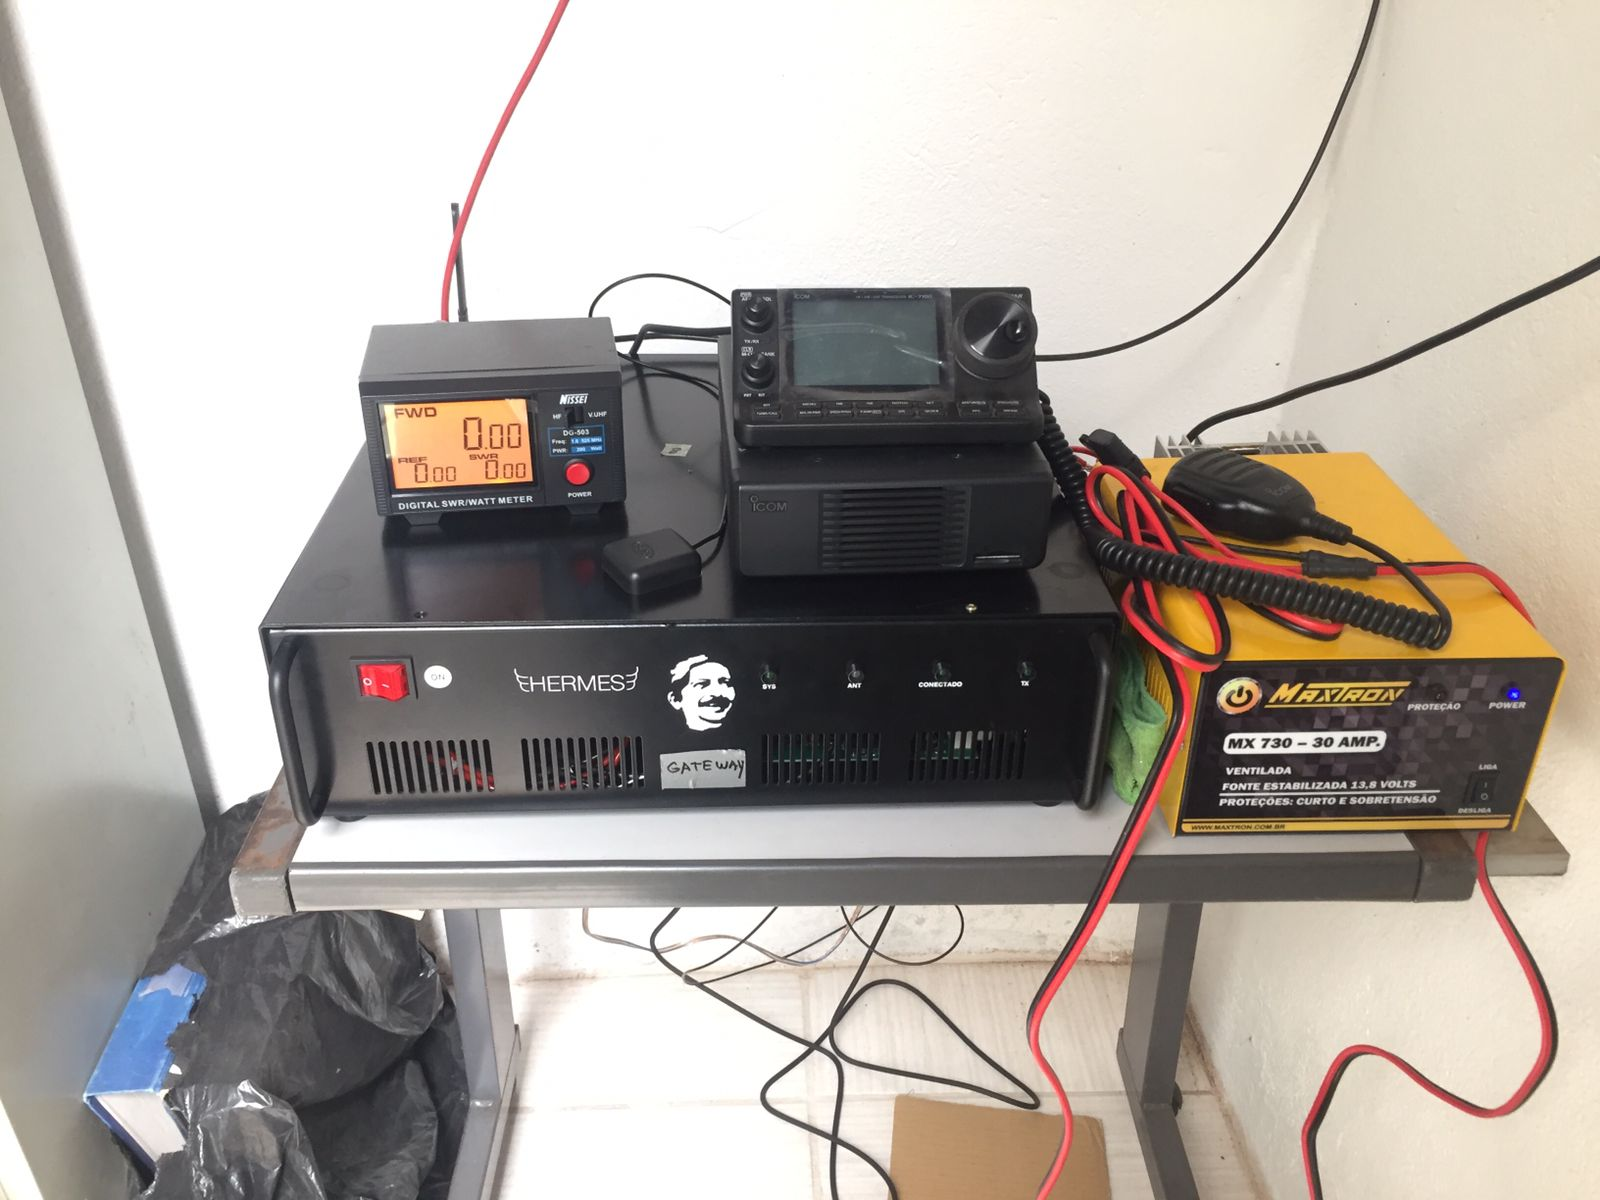
\includegraphics[scale=0.15]{hermes-pic1.jpeg}
  \caption{The HERMES hardware at a ``gateway'' location, a power supply (yellow), a standard HF voice radio (top right) and a wattmeter (top left).}
  \label{fig1}
\end{figure}

\begin{figure}[h!]
  \centering
  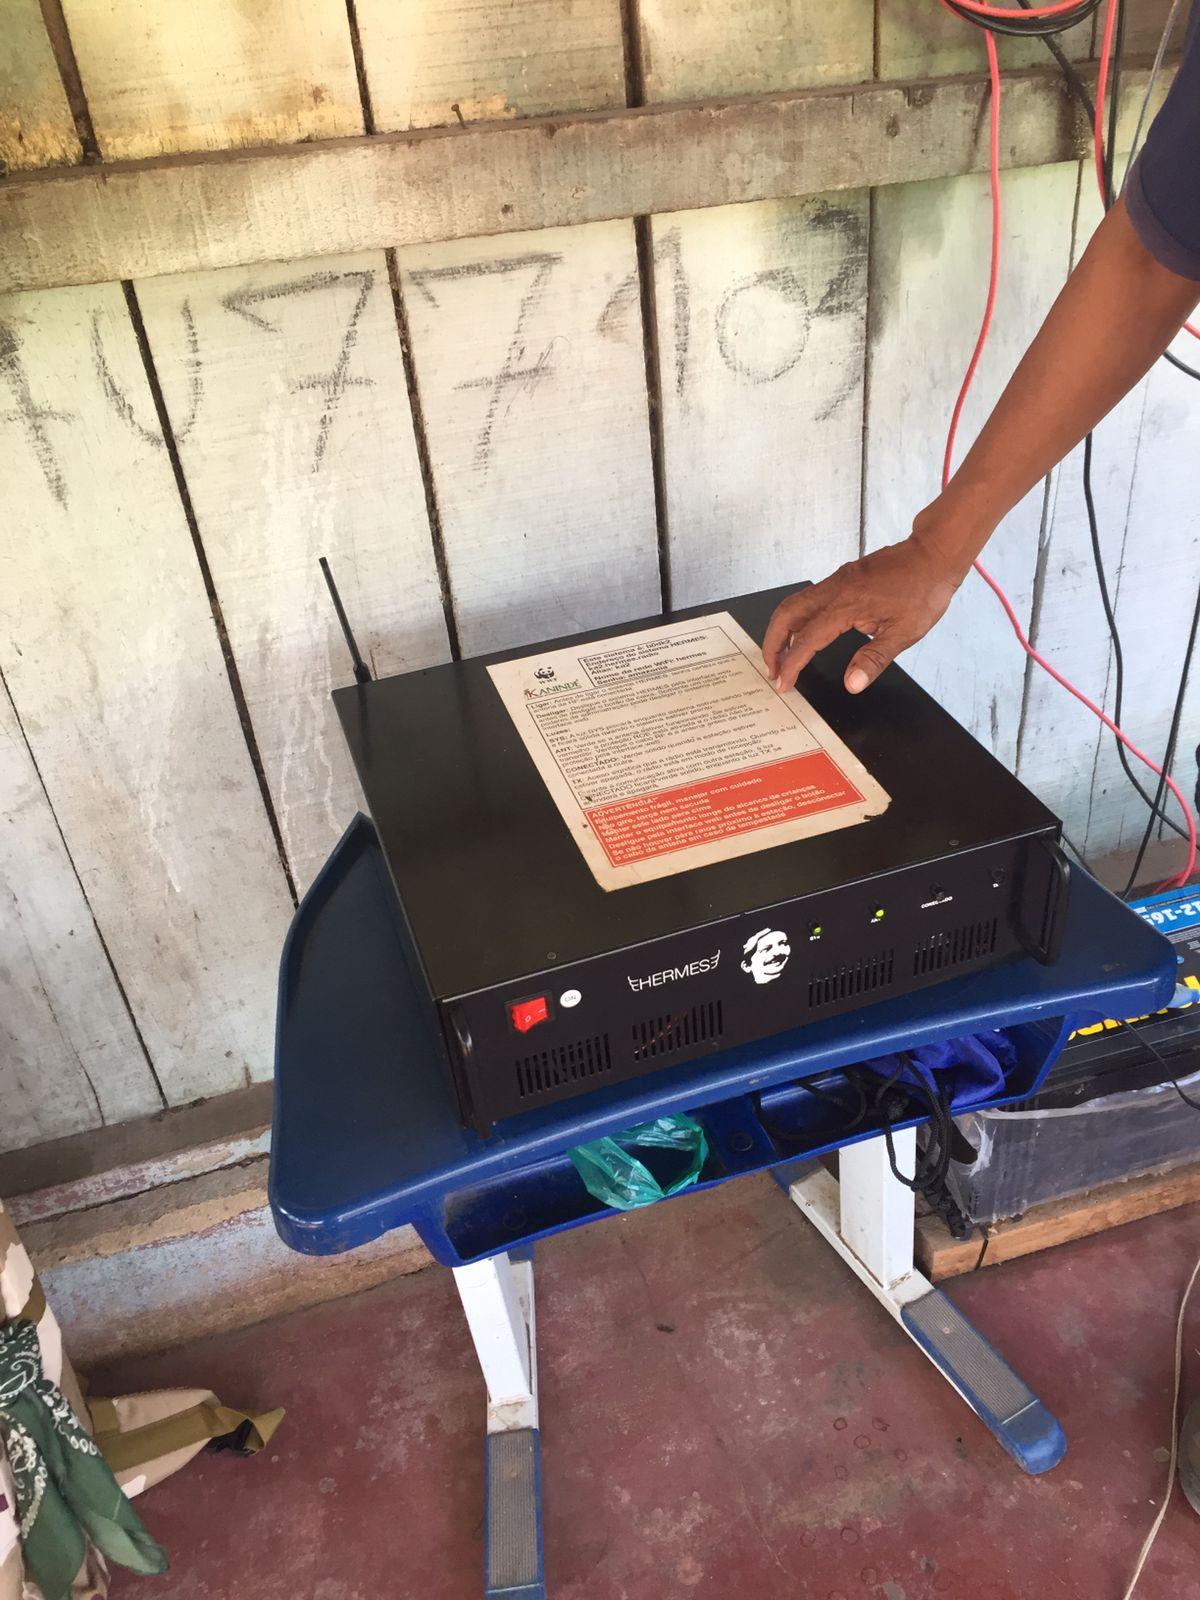
\includegraphics[scale=0.15]{hermes-pic2.jpeg}
  \caption{The HERMES hardware at a ``remote'' location, with a battery appearing the bottom left.}
  \label{fig2}
\end{figure}


HERMES uses GNU UUCP with Debian downstream patches (version 1.07-27 or greater, available at: \url{https://packages.debian.org/bullseye/uucp}).

Specific HERMES network stack source code, radio firmware and other system components are available at:

\begin{itemize}
\item Main network components and firmware: https://github.com/Rhizomatica/hermes-net
\item REST API: https://github.com/Rhizomatica/hermes-api
\item Web GUI: https://github.com/Rhizomatica/hermes-gui
\item Documentation: https://github.com/Rhizomatica/hermes-documentation
\end{itemize}


\section{HERMES Software Stack}

HERMES uses VARA for modem in the current version. Previously it used ARDOP(Amateur Radio Digital Open Protocol).
ARDOP and VARA are
SDR (software defined radio) modems which use modern modulation techniques (OFDM) and support
standard HF transceiver specification (up to 3 kHz bandwidth).

For the network layer, UUCP is used. UUCP is a system for asynchronous
store-and-forward communication first released in Bell Labs Unix V7 in
the late 1970s, and still used today in niches, like communication over HF.

The uucpd (previously called rhizo-uuardop) project was developed to provide
integration between UUCP and the HF modem.

The HERMES network stack is made of:
\begin{itemize}
\item ALSA (Audio/Signal configuration)
\item HF Modem (Modem configuration)
\item UUCP (Network configuration)
\item UUCPD (UUCP / HF Modem connection tools)
\item Graphical Web-based User Interface
\end{itemize}

\subsection{ALSA (Audio configuration)}

Add to ``/etc/asound.conf'':
\begin{verbatim}
pcm.ARDOP {type rate slave {pcm "hw:1,0" rate 48000}}
\end{verbatim}

Where ``hw:1,0'' is the HF transceiver's audio \\

Find your soundcard model(Chip) with the command:
\begin{verbatim}
alsamixer
\end{verbatim}

\begin{figure}[h!]
  \centering
  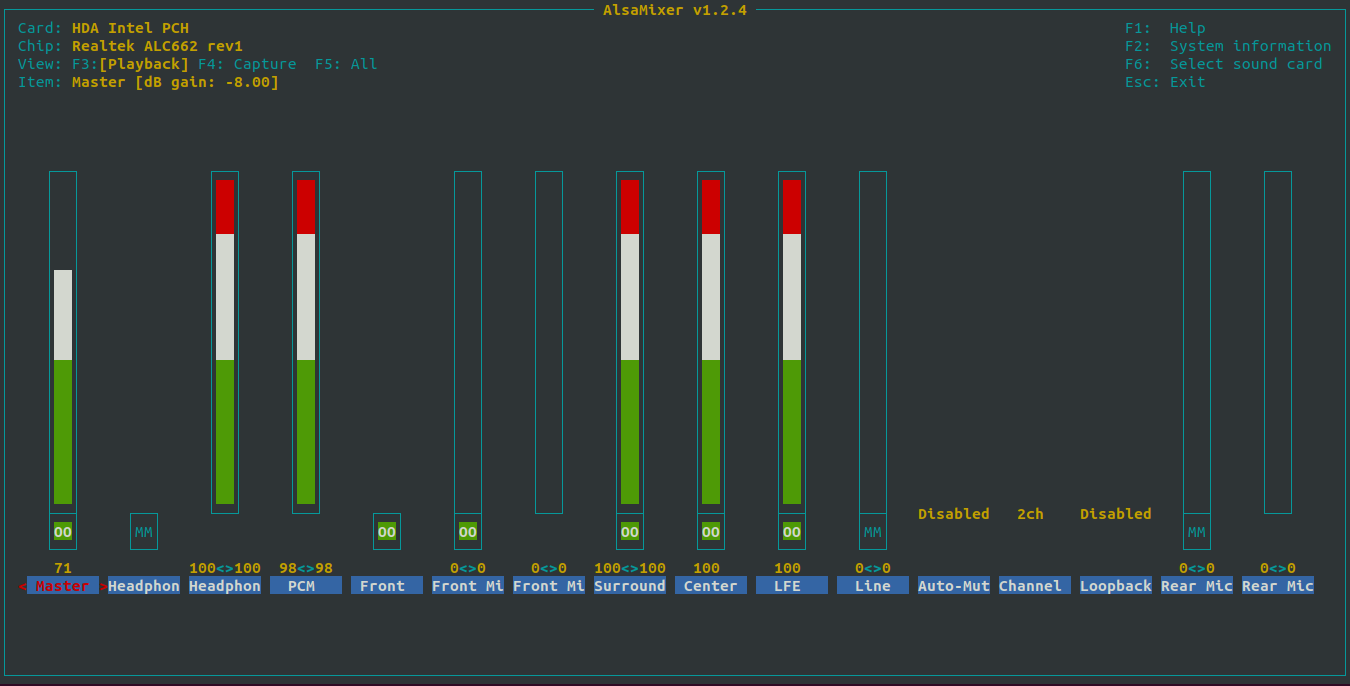
\includegraphics[scale=0.23]{screenshots/software_stack/alsamixer.png}
  \label{fig3}
\end{figure}
  
Set the model on the config file for each station under /stations:

\begin{figure}[h!]
  \centering
  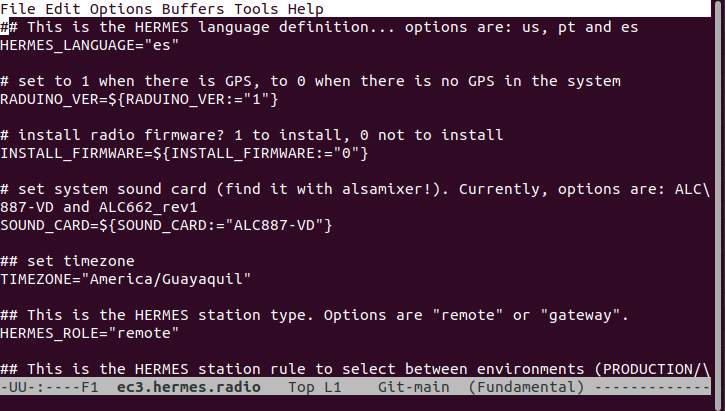
\includegraphics[scale=0.45]{screenshots/software_stack/set_system_soundcard.png}
  \label{fig4}
\end{figure}

\subsection{Modem configuration}
\subsubsection{VARA}
VARA is a High Performance HF modem based on OFDM modulation.
VARA modem is the only piece of private software in the stack.\\
Currently, HERMES uses VARA HF 4.3 or newer as it's standard modem.
Use this protocol with your HERMES if you are looking for best performance available.\\

Please refer to the developer's website for download and instructions on installation and use: \\
\url{https://rosmodem.wordpress.com/}\\

\textbf{Configuration}\\
Edit /opt/VARA/VARA.ini.default to include your license key and callsign.

\subsubsection{ARDOP}

ARDOP is a SDR(software defined radio) modem compatible with both HF and VHF radio transmissions.
The protocol can operate over a wide range of data rates by automatically adjusting for optimized performance under poor multi-path conditions.
Use this protocol with your HERMES if you are looking for a completely open-source and free option.

Download link: \url{https://github.com/DigitalHERMES/ardopc}\\

\textbf{Configuration}\\

The ardop binary should be in /usr/bin/ardop, which can be a
symbolic link to /usr/bin/{ardop1ofdm, ardop2, ardopofdm}.\\

ARDOP service file for the ICOM IC-7100 (USB connection, PTT done over serial):
\begin{verbatim}
[Unit]
Description=ARDOP daemon

[Service]
Type=simple
ExecStart=/usr/bin/ardop 8515 -c /dev/ttyUSB0 ARDOP ARDOP -k FEFE88E01C0001FD -u FEFE88E01C0000FD
ExecStop=/usr/bin/killall -s QUIT ardop
IgnoreSIGPIPE=no
#StandardOutput=null
#StandardError=null
StandardOutput=syslog
StandardError=syslog

[Install]
WantedBy=multi-user.target
\end{verbatim}

Service file when using a VOX based setup (eg. when using an interface like
the Signalink):
\begin{verbatim}
[Unit]
Description=ARDOP daemon

[Service]
Type=simple
ExecStart=/usr/bin/ardop 8515 ARDOP ARDOP
ExecStop=/usr/bin/killall -s QUIT ardop
IgnoreSIGPIPE=no
#StandardOutput=null
#StandardError=null
StandardOutput=syslog
StandardError=syslog

[Install]
WantedBy=multi-user.target
\end{verbatim}


\textbf{Start/stop ARDOP service:}
\begin{verbatim}
systemctl start ardop.service
systemctl stop ardop.service
\end{verbatim}


\textbf{See the log:}
\begin{verbatim}
journalctl -f -u ardop
\end{verbatim}

\subsubsection{Mercury}
Rhizomatica is developing Mercury, a new modem using the latest modulation techniques. It is open-source and currently in development stage. \\
Source code is located at:
\url{https://github.com/Rhizomatica/mercury/}

In the future, HERMES will use Mercury as its standard modem.

\subsection{UUCP (Network configuration)}
UUCP is an acronym of Unix-to-Unix Copy.
It's a protocol for remote execution of commands and transfer of files, email and netnews between computers.

Since HERMES uses Debian GNU/Linux release Bullseye, UUCP packages are installed by default.

If you are not using Debian Bullseye, UUCP Debian package version 1.07-27 or higher should be used, for example,
the version from Debian Bullseye (11):
\url{https://packages.debian.org/bullseye/uucp}

UUCP command line examples follow. To copy a file to a remote host,
the following command adds a copy job to the uucp queue (``-r'' is used to
not start transmission after queuing):
\begin{verbatim}
uucp -C -r -d source.xxx AM4AAB\!/var/www/html/arquivos/${nodename}/
\end{verbatim}

Trigger the transmission of all queued jobs for host
AM4AAA:
\begin{verbatim}
uucico -S AM4AAA
\end{verbatim}

List the jobs:
\begin{verbatim}
uustat -a
\end{verbatim}

Kill a job:
\begin{verbatim}
uustat -k job
uustat -K
\end{verbatim}

See the log:
\begin{verbatim}
uulog
\end{verbatim}


\subsection{UUCPD(UUCP to Modem configuration)}

UUCPD is a set of tools which allow UUCP to use ARDOP or VARA as modem. With this integration, UUCP is fully functional over HF links.

UUCPD comes with two tools: uuardopd and uuport.

UUARDOPD is the daemon which keeps connected to ARDOP or VARA modem and properly receive calls (calling uucico) and initiate calls (uucico calls thought UUPORT connection).

UUPORT is the command invoked by UUCICO (using port type = pipe) when initiating a call (uucico master mode). Communication between uuport and uuardopd is done over shared memory. \\

Download link: \url{https://github.com/Rhizomatica/hermes-net/tree/main/uucpd} \\

\textbf{Install} \\
\\
To compile and install, type:
\begin{verbatim}
  $ make
  $ make install    
\end{verbatim}

\textbf{Configuration} \\
\\
Port configuration example at "/etc/uucp/port":
\begin{verbatim}
  port HFP
  type pipe
  command /usr/bin/uuport    
\end{verbatim}

An alternative Port configuration if you use a patched uucp ( for "\textbackslash Z" support, available in "improved-pipe.patch" which was added to uucp debian package version 1.07-27 ), where uuport pass the callsign of the station to be called to uuardopd with the uucp remote station name (allowing a single uuardopd instance to be used for different remote station callsigns):
\begin{verbatim}
  port HFP
  type pipe
  command /usr/bin/uuport -c \Z
\end{verbatim}

Sys protocol example (tested and works fine) at "/etc/uucp/sys":
\begin{verbatim}
  protocol y
  protocol-parameter y packet-size 512
  protocol-parameter y timeout 540
  chat-timeout 200
\end{verbatim}

Sys configuration example of remote system at "/etc/uucp/sys" (without login prompt):
\begin{verbatim}
  system remote
  call-login *
  call-password *
  time any
  port HFP
  chat "" \r
\end{verbatim}

Sys configuration example of remote system at "/etc/uucp/sys" (with login prompt - should call uuardopd with "-l"):
\begin{verbatim}
  system remote
  call-login *
  call-password *
  time any
  port HFP
  chat "" \r\c ogin: \L word: \P
\end{verbatim}

\textbf{Start/stop UUARDOPD service}
\begin{verbatim}
systemctl start uuardopd.service
systemctl stop uuardopd.service
\end{verbatim}

\textbf{Running uuardopd}\\

Examples of uuardopd invocation:

\begin{verbatim}
$ uuardopd -a 127.0.0.1 -c PU2BBB -p 8515 -t 60 -r ardop
$ uuardopd -a 127.0.0.1 -p 8300 -r vara -o icom -s /dev/ttyUSB0 -f 2750  
\end{verbatim}


\textbf{See the log}
\begin{verbatim}
journalctl -f -u uuardopd
\end{verbatim}

\textbf{UUARDOPD Usage}
\begin{verbatim}
-c callsign:         Station Callsign (Eg: PU2HFF)
-d remote_callsign:  Remote Station Callsign (optional)
-r [ardop,vara]:     Choose modem/radio type
-a tnc_ip_address:   IP address of the TNC
-p tcp_base_port:    TCP base port of the TNC. ARDOP uses ports tcp_base_port and tcp_base_port+1
-t timeout:          Time to wait before disconnect when idling (ARDOP ONLY)
-f features:         Enable/Disable features.
    Supported features ARDOP: ofdm, noofdm (default: ofdm)
    Supported features VARA, BW mode: 500, 2300 or 2750 (default: 2300)
-s serial_device:    Set the serial device file path for keying the radio (VARA ONLY)
-l:                  Tell UUCICO to ask login prompt (default: disabled)
-o [icom,ubitx,shm]: Sets radio type (supported: icom, ubitx or shm).
-h:                  Prints this help
\end{verbatim}

\textbf{UUPORT Usage}
\begin{verbatim}
-c system_name:      Name of the remote system (default is don't change).
-e logfile.txt:      Log file (default is stderr).
-h:                  Prints this help
\end{verbatim}
\subsection{User Web Interface}

HERMES provides a web-based interface for sending messages, files and emails. It also allows for user management and radio configuration, among other features.
Current implementation also supports symmetric cryptography and audio/image compression.

The web app is composed of the front-end interface and a REST API.

\subsubsection{Hermes-GUI}
Hermes-GUI is the front-end interface built with Angular.js.

Source code is located at:
(\url{https://github.com/Rhizomatica/hermes-gui/}).\\

The project was generated with Angular CLI version 13.2.6.
Angular: 13.2.6 Angular CLI: 13.2.6 Node: 12.22.5 Package Manager: npm 8.5.2\\

\textbf{Requirements of the user interface:}

\begin{itemize}
\item ImageMagic: for image manipulation
\item VVC: Best free software low bitrate visual content compression codec: \url{https://github.com/fraunhoferhhi/}
% \item opusenc: para comprimir áudio
\item LPCNet: Best free software audio compression codec: \url{https://github.com/xiph/LPCNet}
\item GnuPG: For cryptography
\item hostapd: WiFi AP mode software
\end{itemize}

The Web interface can be accessed by typing any address in a browser
connected to the WiFi (set the DNS accordingly) or simply 10.0.0.1.\\


\textbf{Install node, npm}\\
Install node preferably(V12.22.5) and npm (node package manager) in your distro

Run 'npm install' inside the project path\\

\textbf{Development server}\\
Configure .env file with your parameters and run npx ts-node setEnv.ts to set .env values in enviroment.ts.

Run ng serve --configuration=en for a dev server in english, you can change the language to spanish (ng serve --configuration=es) or portuguese (ng serve --configuration=pt) if you wish. Navigate to http://localhost:4200/. The app will automatically reload if you change any of the source files.\\

\textbf{Code scaffolding}\\
Run ng generate component component-name to generate a new component. You can also use ng generate directive|pipe|service|class|guard|interface|enum|module.\\

%\textbf{Build & Publish}
%Access remotly machine in port 22 with ssh -p 22 hermes@[my_host_ip] type sudo su to admin verification Set origin main branch git checkout main Update project git pull Create an .env file like a .env.example in root directory Check and configure .env file with your parameters DEV/PROD and run npx ts-node setEnv.ts to set .env values in enviroment.ts. Remove all files in dist folder rm -r dist/ Run npm run build / ng build to build the project. The build artifacts will be stored in the dist directory. Copy them in /var/www/html/ directory cp -a dist/hermes/pt /var/www/html/ cp -a dist/hermes/es /var/www/html/ cp -a dist/hermes/en-US/ /var/www/html/ Done Navigate to HERMES

\textbf{Running unit tests}\\
Run ng test to execute the unit tests via Karma.\\

\textbf{Running end-to-end tests}\\
Run ng e2e to execute the end-to-end tests via Protractor.\\

\textbf{Further help}\\
To get more help on the Angular CLI use ng help or go check out the Angular CLI README.\\

\textbf{Interface Contents}\\
Inside the folder src you will find the angular templates for the system's interface.

On style.less there are the styling code, writen in less.

Inside the app folder, you will find the template components. The app-routing module.ts file is responsible for linking the templates to url adressess. and the app.component, the aplication root template.

For every system component, there will be a folder with the component.html, component.less, and component.ts. On the .html file there is the html angular template, and on the component.ts you will find typescript code related to that component.

Also inside the app folder, there is the \_services foder, where you can find common services shared between the components to access the [station-api] (https://github.com/DigitalHERMES/station-api).

On assets folder you find links to svgs and image files used on the interface design.

On the locale folder there are the xlf files for translation. For the translations, we are using i18n angular module. To generate translations, you need to use ng extract-i18n --output-path src/locale/ to generate the messages,xlf file and then xliffmerge --profile xliffmerge.json pt es to transpose the new data to both messages.es.xlf and messages.pt.xlf, where you can input the new tranlation tokens.

\subsubsection{Hermes-API}
Hermes-API is a REST api for use on Hermes stations to exchange messages between them.
It uses Lumen PHP Framework and composer to manage its own dependencies.\\

Source code is located at:
(\url{https://github.com/Rhizomatica/hermes-api/}).\\

\textbf{Server Requirements:}
\begin{itemize}
  \item Web server
  \item PHP >= 7.3
  \item OpenSSL PHP Extension
  \item PDO PHP Extension
  \item Mbstring PHP Extension
  \item SQLite DataBase\\
\end{itemize}

\textbf{Installation settings}\\

Setup your installation settings creating a .env file from .env.example\\

\textbf{Run Composer}\\

Composer is a dependency manager for PHP.

Run composer in your folder to install the dependencies and update relevant packages:
\begin{verbatim}
COMPOSER_ALLOW_SUPERUSER=1 composer install
COMPOSER_ALLOW_SUPERUSER=1 composer update

\end{verbatim}

\textbf{Copy hermes-api to /var/www/station-api/}\\

Go to your hermes-api folder and run:
\begin{verbatim}
  cp -rT . /var/www/station-api/
\end{verbatim}

\textbf{GNU Privacy Guard}\\

Create the folder for GNU Privacy Guard and change owner:
\begin{verbatim}
mkdir -p /var/www/.gnupg
chmod 700 /var/www/.gnupg
chown www-data:www-data /var/www/.gnupg
\end{verbatim}

\textbf{Setup public folders for UUCP}\\

Create and give permissions to inbox/outbox, downloads and temp folders to uucp public:
\begin{verbatim}
mkdir -p /var/www/station-api/storage/app/inbox
chmod 777 /var/www/station-api/storage/app/inbox
mkdir -p /var/www/station-api/storage/app/outbox
chmod 777 /var/www/station-api/storage/app/outbox
mkdir -p /var/www/station-api/storage/app/downloads
chmod 777 /var/www/station-api/storage/app/downloads
mkdir -p /var/www/station-api/storage/app/tmp
chmod 777 /var/www/station-api/storage/app/tmp
mkdir -p /var/www/station-api/storage/app/uploads
chmod 777 /var/www/station-api/storage/app/uploads
\end{verbatim}

The structure created is used by the app as follows:
/uploads (Files of outgoing messages)
/downloads (Files generated from the inbox received messages)
/inbox (incoming hermes message packs)
/outbox (hermes message pack for deliver)
/tmp (tmp files)\\

\textbf{Link folders}
\begin{verbatim}
ln -sf /var/www/station-api/public/ /var/www/html/api
\end{verbatim}

\textbf{Change owner of the app folder}
\begin{verbatim}
chown -R www-data:www-data /var/www/station-api/ 
\end{verbatim}

create database.sqlite file in database folder

To start a fresh database: php artisan migrate:refresh --seed\\

\textbf{Database setup}\\

Create a database named hermes and user with all privileges:

\begin{verbatim}
  echo "CREATE USER hermes IDENTIFIED BY 'db_hermes'; " > sql_commands.sql
  echo "CREATE DATABASE hermes;" >> sql_commands.sql
  echo "GRANT ALL PRIVILEGES ON hermes.* TO hermes;" >> sql_commands.sql
  
  mysql < sql_commands.sql
\end{verbatim}

Then go to your hermes-api folder and run Artisan for the migrations:
\begin{verbatim}
  cd /var/www/station-api/
  php artisan migrate
  php artisan db:seed    
\end{verbatim}

\textbf{Running on port 8000:}\\

> php -S localhost:8000 -t public\\

\textbf{Hermes Message Pack}\\
Hermes Message Pack is a tar gziped file named .hmp\\

% We use ``/var/www/html/arquivos'' as the default UUCP path to send
% files through the web interface.

%ps: WORK IN PROGRESS

%Email server (MTA) can either run locally or only in a central host with
%Internet. Stations can either opt to connect to a central station on demand,
%have some pre-defined schedule, or the central station connects to the
%community stations doing a pooling, delivering and downloading emails and
%files.

%\subsection{WebPhone}

%WORK IN PROGRESS

%\url{https://gitlab.tic-ac.org/keith/webphone/wikis/hermes}

\end{document}
